\documentclass[fleqn,10pt]{wlscirep}
\usepackage[utf8]{inputenc}
\usepackage{array}
\usepackage{pdflscape}
\usepackage{longtable}
\usepackage{threeparttable}
\usepackage[table]{xcolor}
\usepackage{tcolorbox}
\usepackage{xspace}
\usepackage{xcolor}
\usepackage{graphicx}
\definecolor{heatmap1}{RGB}{8,48,107}    % Dark Blue (High value)
\definecolor{heatmap2}{RGB}{33,113,181}  % Medium Blue
\definecolor{heatmap3}{RGB}{66,146,198}  % Light Blue
\definecolor{heatmap4}{RGB}{107,174,214} % Lighter Blue
\definecolor{heatmap5}{RGB}{198,219,239} % Very Light Blue
\definecolor{heatmap6}{RGB}{237,248,251} % Almost White

%Redline version
\newcommand{\edit}[1]{\textcolor{red}{#1}}
\newcommand{\goedit}[1]{\textcolor{black}{#1}}

\def\ourmetric{\texttt{Spurious Rate}\xspace}


\tcbset{
  palebluebox/.style={
    enhanced jigsaw,     % use the jigsaw engine for flexible breaking
    breakable,           % allow the box to split across pages
    colback=gray!10!white,
    colframe=gray!30!white,
    boxrule=0pt,
    sharp corners,
    width=\textwidth,
    before skip=10pt,
    after skip=10pt,
    left=8pt, right=8pt, top=3pt, bottom=3pt,
  }
}

\usepackage[T1]{fontenc}
\usepackage{makecell}
\title{Measuring Physicians and LLM Relevance Alignment in Medical Question Answering}

% \author[]{Anonymous Author(s)}
\author[1,2 *]{Yuexing Hao, Ph.D.}
\author[1]{Kumail Alhamoud, M.S.}
\author[1]{Hyewon Jeong, M.D., M.S.}
\author[1]{Haoran Zhang, M.S.}
\author[1]{Grace Yan, B.S.}
\author[1]{Isha Puri, B.S.}
\author[3]{Philip Torr, Ph.D.}
\author[6]{Mike Schaekermann, Ph.D.}
\author[2]{Saleh Kalantari, Ph.D.}
\author[4,5]{Ariel D. Stern, Ph.D.}
\author[1]{Marzyeh Ghassemi, Ph.D.}

\affil[1]{Massachusetts Institute of Technology, Cambridge, MA, 02139, USA}
\affil[2]{Cornell University, Ithaca, NY, 14850, USA}
\affil[3]{University of Oxford, Oxford, UK}
\affil[4]{Hasso Plattner Institute, Potsdam, Germany}
\affil[5]{University of Potsdam, Potsdam, Germany}
\affil[6]{Independent Researcher}

\affil[*]{Corresponding Author: yuexing@mit.edu}


\begin{abstract}
Large Language Models (LLMs) have demonstrated strong performance on medical question answering (QA) benchmarks, including standardized medical exams. However, correct answers alone do not guarantee correct reasoning, as a model can reach the right conclusion while attending to input that a clinician would consider irrelevant. Here, we evaluated how physician trainees and LLMs estimate sentence level relevance when answering clinical QA items. We obtained annotations on 933 QA pairs from 53 physician trainees, with a subset independently reviewed by 7 board certified physicians, labeling each sentence of the case description as high relevance, low relevance, or irrelevant. We then compared these expert annotations with LLM-generated relevance labels and measured the effect of restricting the input to the sentences each labeler considered relevant. The average sentence level concordance between LLMs and the physician trainee majority vote ranged from 44.9\% to 65.9\%, while the concordance between physician trainees and board certified physicians was 72.4\%, indicating a modest but consistent gap. Removing sentences that physician trainees judged low relevance or irrelevant increased the accuracy of most LLMs on the four source datasets, and similar gains were observed when each LLM filtered its own input or the input of another model. These results suggest that current LLMs do not consistently prioritize the same case information as physician trainees, and that relevance aware filtering can be a useful probe of model reasoning. The findings are based on multiple choice exam questions and should be interpreted as an evaluation step, rather than direct evidence of readiness for clinical deployment.
\end{abstract}

\begin{document}

\flushbottom
\maketitle

\section{Main}

Large language models (LLMs) have shown strong performance across a range of medical tasks \cite{de2025we}, with systems like GPT-4 \cite{openai_gpt-4_2024} and MedPaLM \cite{singhal2023large} outperforming human averages on standardized medical examinations \cite{cabral_clinical_2024, mcduff_towards_2025, liu2025generalist, holmes2025radonc, van2024adapted}. Multiple LLM companies including OpenAI and Anthropic launched the specific HIPAA-compliance LLMs. However, high performance on exam-style datasets may overstate a LLM’s generalizability~\cite{li_mediq_2024, hao2025large, deng-etal-2024-investigating}, as many tasks do not reflect the complexity of real-world use cases \cite{xia_cares_2024}. In human-facing settings, it is crucial to understand how models filter and prioritize relevant information \cite{park_does_2015}. 

Estimation of contextual relevance is a critical aspect in many applications \cite{KonopaskyArtinoBattistaOhmerHemmerTorreRamanivanMerrienboerTeunissenMcBeeRatcliffeDurning+2020+257+264, sayres2025towards, hao2024outcome}. Techniques such as semantic entropy \cite{farquhar_detecting_2024}, influence functions \cite{choe_what_2024}, context attribution \cite{cohen-wang_learning_2025, liuattribot2024}, and evidence inference \cite{deyoung_eraser_2020} have been employed to assess which elements within a context hold the most importance. Despite these efforts, existing relevance estimations are often imprecise and noisy, with models sometimes producing misleading or overly confident assessments that deviate from human judgment \cite{es_ragas_2024}. Even when estimations appear less noisy, model-generated relevance labels may not concord with those of human experts. This gap is particularly concerning in human-facing domains where alignment with expert judgment is necessary \cite{zhao_moverscore_2019, schuler_context_2025}. 

Models may depend on input features that a clinician would not treat as informative \cite{adam2022mitigating, qazi2025automation}. Prior work has shown that restricting inputs to relevant content can reduce distraction, streamline evidence integration, and lower memory requirements \cite{khattab_baleen_2021, chuang_selfcite_2025, lu_learn_2022, bucinca_trust_2021}. Small, clinically unimportant perturbations of medical questions have also been shown to produce statistically significant shifts in model treatment recommendations \cite{gourabathina2025medium}. To date, however, little work has examined whether models and physicians agree on which case information is worth attending to, or whether concentrating models on such content measurably improves downstream answers.

Characterizing whether LLMs attend to the same input sentences that clinicians treat as informative is a useful step toward understanding how these models derive their answers \cite{strong_chatbot_2023, katz_gpt_2024}. Such comparisons can complement accuracy based evaluation by flagging cases where a correct answer is accompanied by reliance on sentences that clinicians would not regard as decisive \cite{chiang_can_2023, McCoy_NEJM_SCTBenchmark}. Alignment between model attributed and clinician identified evidence has also been proposed as one of several factors relevant to clinician trust in diagnostic AI tools \cite{huang2025trustworthiness, huang2026probellm}. Restricting LLMs to sentences that clinicians judge highly relevant provides an auditing lens to probe whether model predictions depend on content that humans consider peripheral \cite{zhou_explainable_2025, wu_medreason_2025, bansal_does_2021}. Such dependencies do not always reduce benchmark accuracy, but they can complicate the interpretation of benchmark performance.

A related concern is that LLMs may be trained on data that overlap with public medical benchmarks. Relevance aware filtering does not by itself distinguish memorization from genuine reasoning, but it offers one additional axis along which such effects can be examined. In our setting the four source datasets span release dates from 2020 to 2025, so the potential for training set contamination varies across subsets and we treat this as a confound rather than a controlled variable.

To study how physician trainees and LLMs interpret the relevance of input patient context, we curate \emph{MedPAIR} (\underline{Med}ical \underline{P}hysician trainee and \underline{AI} \underline{R}elevance), a dataset that pairs sentence level relevance annotations from physician trainees with LLM derived relevance labels on the same QA items. We use this dataset to run an empirical study of relevance misalignment. Three research questions organize the study. First, to what extent do physician trainees and contemporary LLMs agree on which sentences of a clinical vignette matter for its question? Second, does restricting an LLM's input to sentences that physician trainees label highly relevant change downstream answer accuracy, and how should such changes be interpreted given potential confounds? Third, can an LLM's own sentence level relevance scores drive comparable filtering effects, so that the approach does not depend on human annotation at inference time? Medical QA datasets are a primary method of evaluating LLM performance in clinical tasks \cite{pal_medmcqa_2022, zhang_survey_2024, jin_rjua-meddqa_2024, soni_radqa_2022}, yet existing resources primarily score final answers and do not track which parts of the case the model or the human relied on \cite{toma_clinical_2023, adlakha_evaluating_2024, bedi2026medhelm}. Recent work on explanation generation and qualitative reasoning analyses focuses on the reasoning produced after the input context has already been interpreted \cite{khandekar2024medcalc}.
%To improve our understanding of what context in the QA that LLM used for answering, we first need a comparison study between domain experts and LLM's relevance labels and measure its alignment. % Recent work has argued that the absence of expert-annotated reasoning data limits the development of reliable models  \cite{zhou_explainable_2025, tang_medagents_2024}. 

We collect sentence-level relevance labels on 933 samples drawn from four source datasets - \textit{Massive Multitask Language Understanding}  (MMLU)-precision medicine (192 QAs) \cite{hendrycks_measuring_2021}, \textit{Medbullets} (160 QAs), \textit{JAMA Clinical Challenge dataset} (295 QAs) \cite{chen_benchmarking_2025}, and \textit{MedXpertQA} (286 QAs) \cite{zuo_medxpertqa_2025} - from 53 physician trainees. Physician trainees annotations are verified by a group of seven physician experts to ensure the reliability of their labels.
We generate LLM relevancy labels in two ways. First by prompting all LLMs (GPT-4o \cite{hurst2024gpt} and GPT-5 \cite{singh2025openai}, MedGemma-27B \cite{sellergren2025medgemma}, Qwen2.5-14B-Instruct, Qwen2.5-72B-Instruct \cite{qwen_qwen25_2025}, and Llama-3.1 70B-Instruct \cite{grattafiori_llama_2024}) to self-report sentence-level input relevance~\cite{choi_identifying_2024, wang-etal-2025-medcite}. We also use ContextCite \cite{cohen-wang_contextcite_2024} to retrieve sentence-level relevancy from the four open-source LLMs tested. 
%ContextCite is a context attribution framework that reversely maps model outputs to the input sentences which are most responsible for their generation. This approach allows us to quantify the degree of alignment between human and model assessments of contextual importance. 


Our empirical study addresses these questions along three axes. First, we measure sentence level concordance. Board certified physicians agree with the physician trainee majority vote at 72.4\%, while LLM concordance with the same reference ranges from 44.9\% to 65.9\%. Second, we examine how restricting the input to the sentences each labeller marked as highly relevant affects downstream QA performance, and find that most LLMs gain accuracy after this filtering, whether the filter is derived from physician trainee labels or from another LLM. Third, we quantify a \ourmetric per model, defined as the fraction of originally correct answers that become incorrect once physician trainee identified low or irrelevant sentences are removed. This rate ranges from 5.8\% to 24.8\% in our sample and is best read as a proxy for reliance on content that physician trainees did not consider decisive, rather than as a direct measure of spurious reasoning. Our contribution is therefore an empirical characterisation of how current LLMs and physician trainees diverge on sentence level relevance in clinical QA, alongside the release of \emph{MedPAIR} as the paired annotation dataset that enables this and subsequent analyses.  %Our full workflow can be found in Figure \ref{fig:study_design}.

\section{Results}
\subsection{The MedPAIR dataset and study design}

\subsubsection{Medical QA Dataset Construction}
To examine the alignment between physician trainees’ and LLMs’ assessments of relevance, we concentrate on existing QA pairs grounded in specific patient case scenarios, rather than general evidence-based questions. We draw on four source datasets: \textit{Massive Multitask Language Understanding}  (MMLU)-precision medicine (released September 2020)\cite{hendrycks_measuring_2021}, \textit{Medbullets} (released March 2021), \textit{JAMA Clinical Challenge} (items collected from July 2013 to October 2023)\cite{chen_benchmarking_2025}, and \textit{MedXpertQA} (released January 2025) \cite{zuo_medxpertqa_2025}. The Medbullets and JAMA papers were preprinted in April 2025, and JAMA items require paywall access. The characteristics for each dataset are presented in Supplementary Information. Each source provides multi-sentence patient case descriptions paired with questions (4-option or 10-option multiple-choice) and answers, offering a rich context for relevance annotation. Such patient vignettes are broadly recognized in the medical and social sciences, including health economics, and physician responses to clinical vignettes have been shown to predict realized billing behavior in the U.S. Medicare system \cite{cutler_physician_2019}. We obtained approval from the MIT Committee on the Use of Humans as Experimental Subjects (IRB: 2504001610) and preregistered our dataset collection protocol on the Open Science Framework (OSF) \cite{hao_alhamoud_jeong_puri_torr_kalantari_schaekermann_stern_ghassemi_2025}. No personally identifiable patient information was involved in this study.

%Each QA presents a detailed vignette, which is often a long case description covering patient demographic information, symptoms, exam findings, family history, etc. 
%From a combined pool of 4,052 QA pairs, we constructed the final dataset by randomly sampling 250 pairs each from MMLU and Medbullets, and 750 pairs each from JAMA and MedXpertQA, resulting in a curated dataset of 2,000 QA pairs. By pooling these sources, \emph{MedPAIR} covers a wide spectrum of clinical topics and difficulty levels, ensuring that the evaluation is robust across various scenarios from routine to rare conditions. 

\begin{table}[h!]
\centering
\normalsize
\setlength{\tabcolsep}{10pt} 
\begin{tabular}{l|l|c|c|c|c}
\toprule
\textbf{Dataset} & \textbf{Data Source} & \textbf{Total QA} & \textbf{\makecell[c]{Total\\ Options}} & \textbf{\makecell[c]{Avg\\ Sentence}} & \textbf{\makecell[c]{Physician-Labeled\\ Low/Irrelevant Sentence (\%)} }\\
\toprule
\midrule
\textbf{\makecell[l]{MMLU \\{\small(Precision Medicine)}}}  & Medical textbooks & 192 & 4 & 15.9 {\small(7.0)} & 39.5\% \\\hline
\textbf{\makecell[l]{JAMA \\ Clinical Challenge}}  & Journal articles & 295 & 4 & 26.8 {\small(8.5)} & 35.0\% \\\hline
\textbf{MedBullets}  & USMLE & 160 & 4 & 21.0 {\small(4.6)} & 40.5\% \\\hline
\textbf{MedXpertQA}  & Licensing Exam & 286 & 10  & 14.9 {\small(5.6)} & 32.8\% \\
\bottomrule
\textbf{Overall}  &   & 933 & 4/10 & 21.3 {\small(8.8)} & 36.1\% \\
\bottomrule
\end{tabular}
\vspace{0.7mm}
\caption{\textbf{Comparative Analysis of Physician Trainee–Annotated \emph{MedPAIR} Dataset Characteristics.} Values in parentheses represent standard deviations.}
\label{tab:comparison_1}
\end{table}


\begin{figure}[h!]
  \centering
  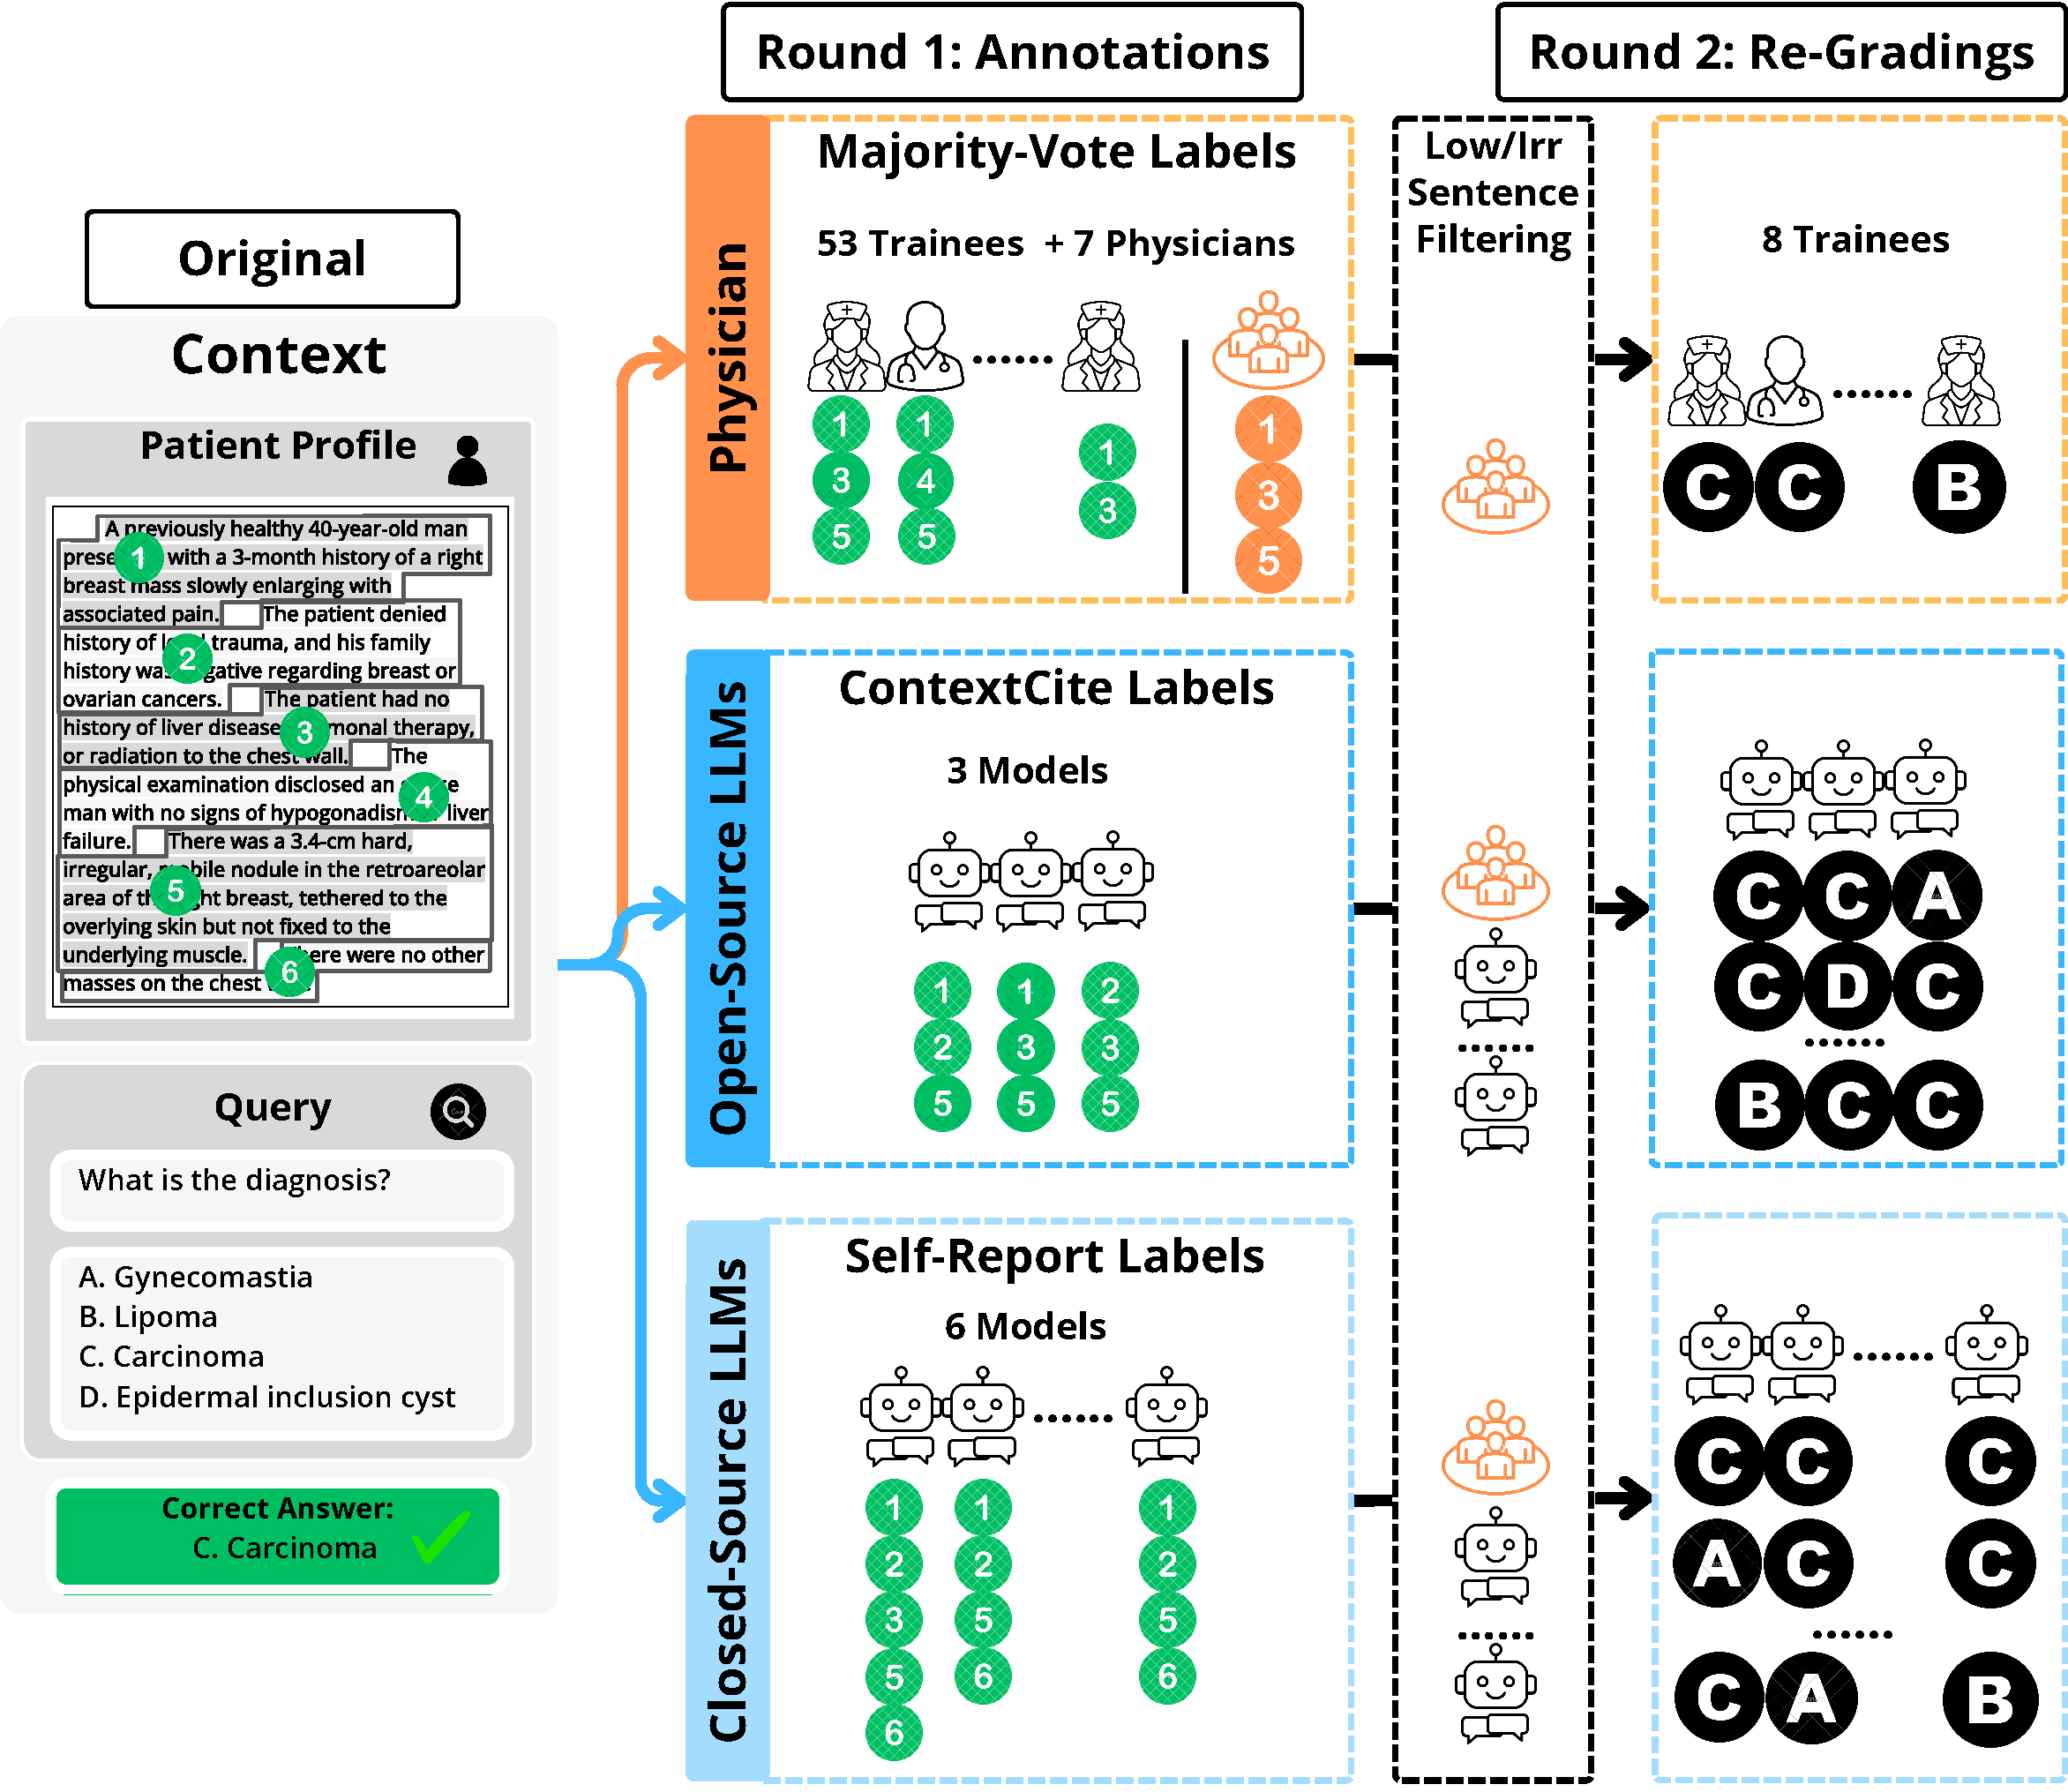
\includegraphics[width=0.9\textwidth]{Figures/MedPAIR-Nature.pdf}
  \caption{\textbf{Study Design.} }
  \label{fig:study_design}
\end{figure}

Across the four datasets, there are 4,052 QA pairs in total. We first remove 2,052 pairs in which the patient profile contains two or fewer sentences. We then exclude 629 pairs that have one or no correct answers, as well as 448 pairs that require information from modalities other than text. This leaves us with a set of 933 QA pairs to obtain labels on.  
We use an online commercial labeling platform to recruit 52 physician trainees, generating a total of 6,224 QA labels on the 2,000 QA pairs. 
We remove all questions that no PT can answer correctly (448 pairs), leaving us with 933 QA pairs. 
%Only 2,918 labels answer the step 1 classification correctly (Figure \ref{fig:study_design} panel B). 
% We also remove QAs which PT label as containing only highly relevant sentences, as there would be no impact from low or irrelevant sentences removal (104 QA). The final set of QAs is 1,267.
 
The four QAs have different characteristics, as JAMA Clinical Challenge are usually long and have lots of details, with each sentence containing more words on average. The low relevance and irrelevant sentences also show the characteristics in perplexity that they are harder to predict as they are more complex, less structured, or diverge from typical language patterns the model has seen during training.
%Figure \ref{fig:study_design} shows the \emph{MedPAIR} data curation process.

\subsubsection{Physician Review of Physician Trainee Labels}

Because board certified physicians could not annotate the full dataset, we used a smaller physician review to check whether the physician trainee labels were a usable reference for downstream analyses, rather than to construct an independent gold standard. To compare the two groups, we aggregated the trainee labels on each sentence into a single majority vote and compared it with the label assigned by a board certified physician. The average sentence level matching rate between the physician trainee majority vote and the reviewing physicians was 72.0\% (median 73.7\%, SD 17.7\%, 95\% CI [0.710, 0.730]). A cumulative distribution of these matching rates is presented in the Appendix. We treat this value as a measure of trainee physician agreement rather than of trainee accuracy, since the physicians themselves represent a small cohort and inter physician disagreement is not separately estimated in this review.

We refer to QA items for which the physician trainee physician matching rate falls below 20\% as ambiguous cases and retain them in the dataset so that this subgroup can be analysed separately. Where the downstream analyses in this paper treat the physician trainee majority vote as a reference, this choice is a pragmatic one driven by scale, and the resulting concordance and filtering results should be interpreted against the 72.0\% trainee physician agreement ceiling.

% \subsubsection{Qualitative Feedback from Physician}

A board-certified physician, HJ, reviewed the physician-annotated majority-vote outcomes. Analysis of high- and low-relevance labels reveals that text marked as highly relevant by the physician trainee contains more anatomical structures and comparative descriptions (e.g., progressive, increased), whereas low-relevance text includes more historical information (medication, allergy, travel, social (smoking, illicit drug), etc.) and negative findings (uncomplicated, noncontributory, etc.). %(Table \ref{tab:keyword_readability})

From the full dataset, 30 QA pairs were randomly selected and Dr. HJ compared the original and edited versions after removing irrelevant sentences. The removed low relevance or irrelevant sentences were then grouped into thematic categories, including \textit{1) Redundant Clinical Details}, \textit{2) Negative Result} that is not essential for the current chief complaint, \textit{3) Low or Irrelevant Temporal Information}, and \textit{4) History (Medical, Surgical, Medication, Social) with No or Very Low Clinical Information}. The validation exercise evaluated whether the remaining highly relevant sentences maintained the link to the correct answer and whether removing low-relevance content affected answer correctness. The sample case study and validation sheet are presented in Supplementary Information.

% THIS IS ABOUT WHAT GETS LABELED AS RELEVANT FROM SUBSET, NOT ABOUT THE DATA BEING OKAY TO SUBSET
We compared the final 933 QAs in \emph{MedPAIR} on their average number of sentences, words per sentence, and perplexity. Across the four medical QA datasets, the highly relevant sentences are consistently longer and more uniform in structure, with lower perplexity values and thus greater linguistic predictability. In contrast, irrelevant or low‐relevance sentences were shorter on average, displayed much higher variability in length, and proved more difficult for the language model to anticipate. The specific perplexity details are presented in the Supplementary Material. %There is a clear distinguish between the high and low/irrelevant sentences.

To compare the continuous ContextCite scores produced by the open source LLMs with the ternary labels assigned by the physician trainees, we mapped the numerical scores into the same three category scheme. For each QA pair, we let $k$ equal the number of sentences marked highly relevant by the physician trainee majority vote. We then ranked the sentences by their ContextCite scores, assigned the top $k$ to \textit{high relevance}, and split the remaining sentences between \textit{low relevance} and \textit{irrelevant} using the corresponding trainee counts. This procedure aligns the LLM and human label distributions per item, which makes concordance directly interpretable in terms of which sentences each source considers most important. A consequence is that the total number of sentences placed in each category is held fixed across labellers for a given QA, so the resulting concordance rates reflect the ordering produced by each method rather than differences in how many sentences each method would otherwise label as relevant. We therefore treat concordance in this paper as a measure of ranking agreement, and discuss the sensitivity of concordance to alternative thresholding choices in the Supplementary Information.

\subsection{Humans and LLMs Disagree on Information Relevance}

With the physician trainee labels characterised against a small physician review cohort and the LLM attribution scores mapped onto the same ternary scheme, we next asked how often physician trainees and LLMs agreed on which sentences carry weight for a given QA. This is an alignment question rather than a test of which labels are clinically correct, since the reviewing physicians themselves agree with the physician trainee majority vote only 72.0\% of the time.

\begin{figure}[h!]
  \centering
  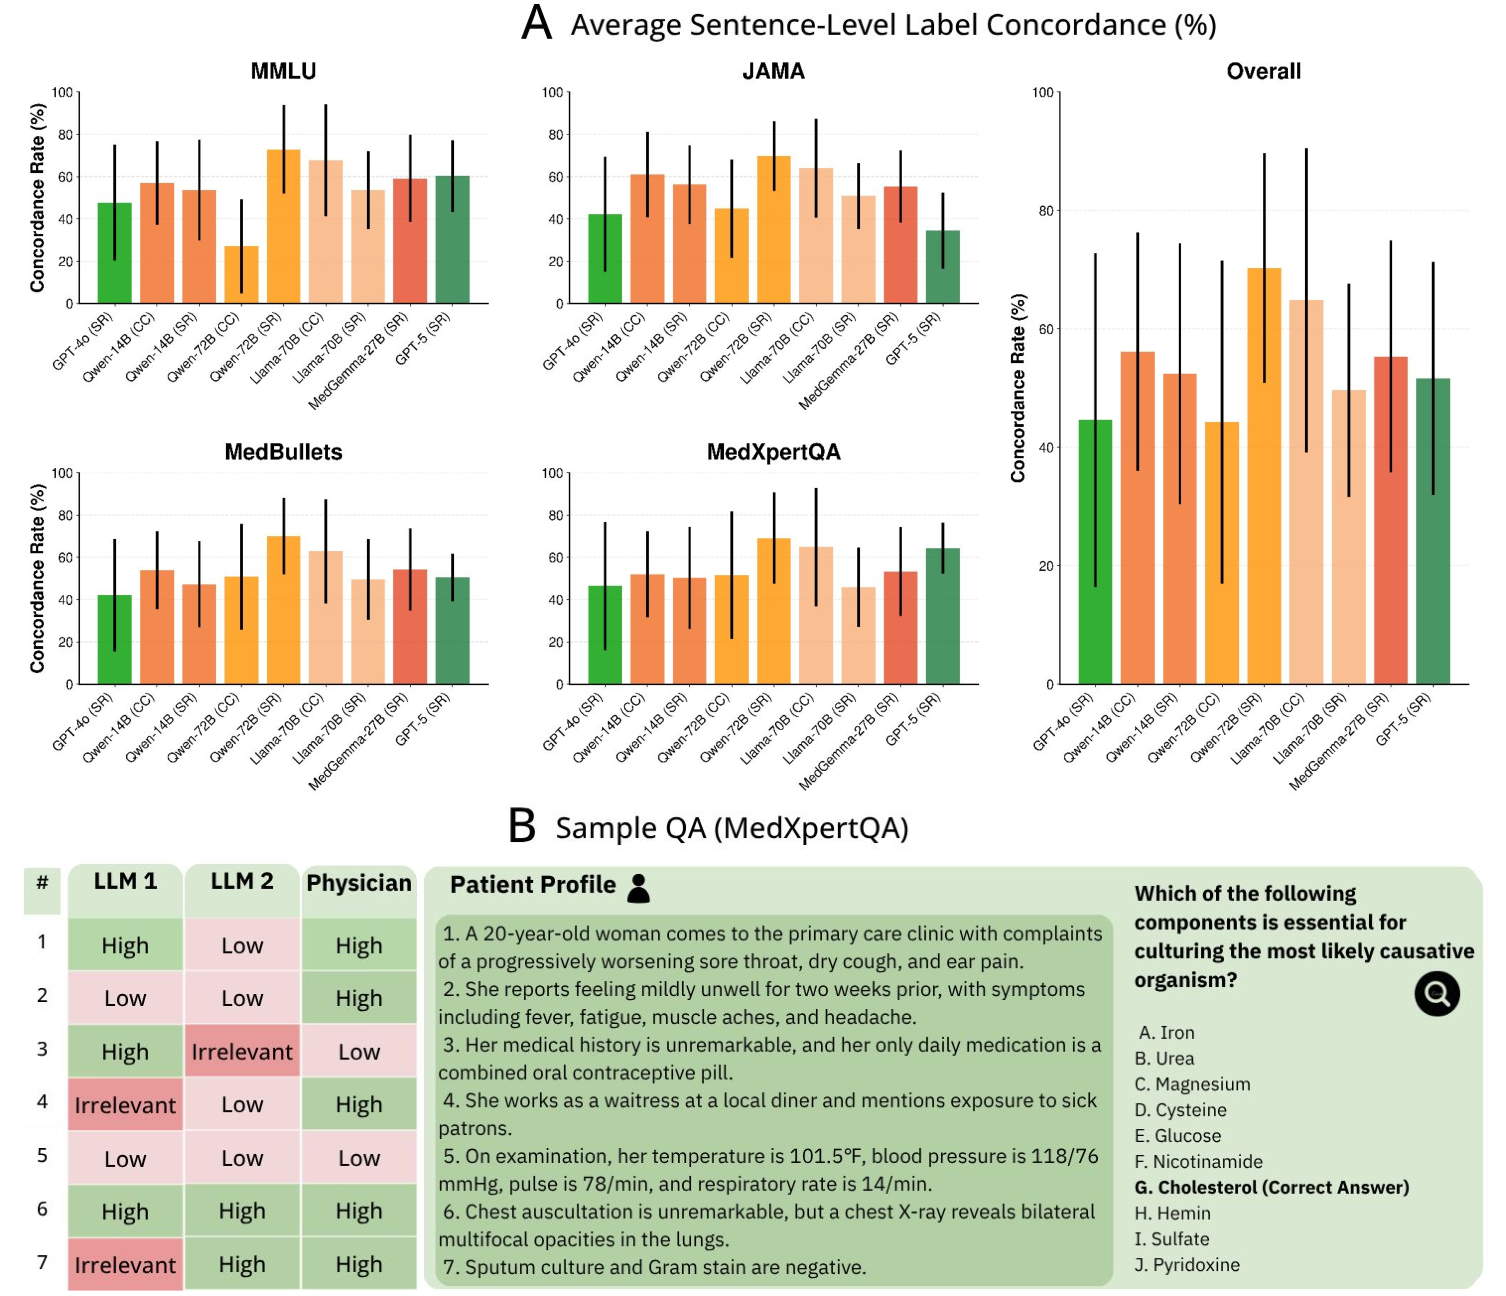
\includegraphics[width=\textwidth]{Figures/Concord_Rate_Sample.pdf}
  \caption{\textbf{Average Sentence-Level Label Concordance (\%)}. Panel A shows the sentence-level concordance between physicians and LLMs is highly variable across datasets and models. Physician Concordance is calculated as inter-rater reliability between physician and majority vote PT across all available labels (2-8 clinical labels). For LLMs, “CC” denotes the ContextCite score; “SR” denotes Self-Reported labels. Panel B shows a sample MedXpertQA QA, which is labeled by physician and LLMs on each sentence. }
  \label{concordance}
\end{figure}

By examining cases in which physician trainees and LLMs produced differing relevance annotations, \emph{MedPAIR} surfaces differences in how each source prioritises patient case information. We quantified the agreement between sentences marked highly relevant by the physician trainee majority vote and those highlighted by the models, using ContextCite scores for Qwen-14B, Llama-70B and Qwen-72B alongside GPT-4o self-reporting. The best performing model, Llama-70B, reached a mean agreement of 65.9\%, below the 72.0\% trainee physician agreement rate but not dramatically so. Roughly a third of sentences that physician trainees considered highly relevant were placed outside the top $k$ sentences by at least one of the models. These gaps narrow the claim from one of stark misalignment to one of consistent but moderate disagreement, and any downstream effect on QA accuracy must be read in that light. The full per-dataset and per-model breakdown is shown in Figure~\ref{concordance}.


A common pattern was overattention to superficial cues. For example, a model might latch onto a laboratory value that is extreme and assume it must be important, even if it is not relevant to the question at hand. %In one case, an LLM fixated on an incidental finding (“mild elevation in liver enzymes”) when diagnosing a skin rash, marking that sentence as relevant and incorporating it into its answer explanation – a form of distractor usage. The human annotators, by contrast, recognized that the rash diagnosis had nothing to do with the liver enzyme quirk and flagged that sentence as irrelevant. Such cases reveal how an LLM’s internal heuristics (e.g. “unusual values are important”) can mislead its reasoning, whereas human experts apply informed judgment to filter out red herrings. 
Conversely, models sometimes missed subtle but crucial cues that humans tagged as relevant. %For instance, a single sentence mentioning “\textit{recent travel to the Ohio River Valley}” in a patient’s history is a critical clue for a fungal infection diagnosis, physician labelers spot it immediately as a key piece of context, but a LLM might ignore it if it hasn’t connected that region with certain infections in its knowledge. These misses show that even highly knowledgeable LLMs may fail to connect the dots in context, especially when the clue requires integrating world knowledge in a non-obvious way.
These findings could be partially due to LLMs occasionally attribute incorrect answers on misinterpreted or irrelevant context, indicating flawed input context relevance estimates. ContextCite highlights cases where a model justifies its answer by citing a sentence it wrongly deems supportive, what researchers term contributive attribution. %For instance, a model might recommend an inappropriate treatment due to a misread clinical detail. These discrepancies between model-perceived and expert-validated relevance expose critical gaps in reasoning.

%By surfacing such divergences, \emph{MedPAIR} pinpoints where models over-rely on spurious cues or fail to distinguish key from peripheral information. These insights offer actionable targets for refining models or prompts, such as encouraging more deliberate evidence selection or filtering superficial correlations.

% \begin{table}[]
% \begin{tabular}{l|ll|ll|l}
% \toprule
%  & \multicolumn{2}{c|}{Self-Report} & \multicolumn{2}{c|}{ContextCite} & Spurious Factors \\
%  \midrule
% Data Source & \begin{tabular}[c]{@{}l@{}}Recall \\ (TPR)\end{tabular} & Kendall $\tau$ & \begin{tabular}[c]{@{}l@{}}Recall \\ (TPR)\end{tabular} & Kendall $\tau$ &  \\
% \midrule
% MMLU &  &  &  &  &  \\
% JAMA &  &  &  &  &  \\
% MedBullets &  &  &  &  &  \\
% MedXpertQA &  &  &  &  &  \\ \hline
% Overall &  &  &  &  & \\
% \bottomrule
% \end{tabular}
% \caption{\textbf{Data Analysis.} TPR indicates True Positive Rate.}
% \label{Confusion_Matrix}
% \end{table}

% \begin{table}[h!]
% \centering
% \resizebox{\textwidth}{!}{%
% \begin{tabular}{l|cc|cc|cc|cc|cc}
% \toprule
% & \multicolumn{2}{c|}{\makecell[c]{MMLU \\ Precision Medicine \\ (250 QAs)}} 
% & \multicolumn{2}{c|}{\makecell[c]{JAMA \\ Clinical Challenge \\ (750 QAs)}} 
% & \multicolumn{2}{c|}{\makecell[c]{Med Bullets \\ (250 QAs)}} 
% & \multicolumn{2}{c|}{\makecell[c]{MedXpertQA \\ (750 QAs)}} 
% & \multicolumn{2}{c}{\textbf{\makecell[c]{Overall \\ (2000 QAs)}}} \\
% \midrule
% & Before & After & Before & After & Before & After & Before & After & Before & After \\
% \midrule
% Qwen-14B     & Acc \% [Std] & -- & -- & -- & -- & -- & -- & -- & -- & -- \\
% GPT-4o     & 1.00 [1.69] & 0.49 [0.85] & 1.75 [2.55] & 0.88 [1.33] & 1.93 [2.09] & 0.94 [1.05] & 1.06 [2.08] & 0.53 [1.05] & 1.42 [2.26] & 0.71 [1.16] \\
% LLaMA-70B    & 77.94\% [0.42] & -- & 48.07\% [0.50] & -- & 48.66\% [0.50] & -- & 14.86\% [0.36] & -- & 30.04\% [0.46] & -- \\
% Qwen-72B    & 89.34\% [0.31] & -- & 57.93\% [0.50] & -- & 62/42\% [0.49] & -- & 16.16\% [0.37] & -- & 35.13\% [0.48] & -- \\
% \bottomrule
% \end{tabular}
% }
% \caption{Number of Irrelevant Sentences}
% \label{tab:comparison}
% \end{table}

% \newpage
% % \section{Sample QA Case Study}
% \label{sample}
% \begin{tcolorbox}[colback=blue!3!white, colframe=blue!50!white, title=Example of QA Data (from MedXpert QA), left=10mm, breakable]
% \small

% \textbf{Patient Profile:} % ++-; +--; -+0; +-0; ---; +++; +-+; FIND HUMAN low/irr but GPT-4o relevant
% \begin{enumerate}
%   \item A 20-year-old woman comes to the primary care clinic with complaints of a progressively worsening sore throat, dry cough, and ear pain.
%   \item She reports feeling mildly unwell for two weeks prior, with symptoms including fever, fatigue, muscle aches, and headache.
%   \item  Her medical history is unremarkable, and her only daily medication is a combined oral contraceptive pill.
%   \item She works as a waitress at a local diner and mentions exposure to sick patrons.
%   \item On examination, her temperature is 101.5℉, blood pressure is 118/76 mmHg, pulse is 78/min, and respiratory rate is 14/min.
%   \item Chest auscultation is unremarkable, but a chest X-ray reveals bilateral multifocal opacities in the lungs.
%   \item Sputum culture and Gram stain are negative.
% \end{enumerate}

% \bigskip
% \textbf{Question: }Which of the following components is essential for culturing the most likely causative organism?


% \bigskip
% \textbf{Options:}
% \begin{enumerate}[label=\Alph*.]
%   \item Iron 
%   ...
%   % \item Urea 
%   % \item Magnesium
%   % \item Cysteine 
%   % \item Glucose 
%   % \item Nicotinamide 
%   % \item Cholesterol  
%   % \item Hemin 
%   % \item Sulfate 
%   \item Pyridoxine
% \end{enumerate}

% \bigskip
% \textbf{Correct Answer:} (G) Cholesterol

% \noindent
% \label{tab:sample_case_label}

% \medskip
% \centering
% \setlength{\tabcolsep}{4pt}
% \begin{tabular}{|l|l|l|l|}
%   \toprule
%   Sentence \# & Physician Labels & GPT4o Self-Reported Labels & MedGemma-27B Labels \\
%   \midrule
%   1 & High & High & Low\\
%   2 & High  & Low  & Low\\
%   3 & Low  & High & Irr\\
%   4 & High  & Irr  & Low \\  
%   5 & Low  & Low  & Low\\
%   6 & High  & High & High\\
%   7 & High  & Irr  & High \\    
%   \bottomrule         
% \end{tabular}
% \end{tcolorbox}


\subsection{Removing Irrelevance Sentences Improves LLM Performance}

Given the moderate disagreement between physician trainees and LLMs on what counts as relevant, we next examined whether restricting models to physician trainee identified relevant sentences shifts their answers. Removing the sentences that physician trainees marked as low relevance or irrelevant raised accuracy for most LLMs on most datasets. We read this as a filtering effect that is consistent with, but not uniquely explained by, reduced distraction from content the physician trainees did not consider decisive. Input length, exposure of memorised strings, and the deliberate inclusion of distractors in USMLE style items are also modified by this intervention, and we return to these confounds in the Discussion. Physician trainee labelling instructions explicitly stated that the QA should be answerable from the highly relevant sentences alone, so the filtering operation at least preserves the sentences that a physician trainee would identify as sufficient.

\begin{figure}[h!]
  \centering
  \includegraphics[width=\textwidth]{Figures/MedPAIR_Result_combined.pdf}
  \caption{\textbf{Effect of Filtering Context on Final Performance.} Figure illustrates how accuracy shifts on four medical benchmarks (MMLU, JAMA, MedXpert, MedBullets) when utilizing various sets of LLMs-labeled highly relevant sentences. Solid black horizontal lines denote the original baseline accuracy, while dotted lines represent the highest accuracy achieved. Colored shapes indicate performance when specific models (GPT-4o, GPT-5, Qwen-14B and Qwen-72B, Llama-70B, MedGemma-27B, Trainee, Physician) highly-relevant sentences are used in predictions. Percentage annotations highlight the largest improvement or decline between the baseline and the best observed accuracy.}
  \label{results}
\end{figure}

Figure \ref{results} shows that removing sentences that physician trainees considered low relevance or irrelevant is associated with higher accuracy for most LLMs. The per dataset improvements vary in size and direction, and we report them here as observed differences rather than statistically tested effects. The Round 2 subset contains only 248 QA pairs, so we do not attach confidence intervals or significance tests to the per dataset changes in Figure~\ref{results}. Qwen-72B’s accuracy rises from 89.3\% to 92.2\% on MMLU Precision Medicine and from 35.1\% to 62.2\% overall, while GPT-4o moves from 95.6\% to 96.4\% and from 39.3\% to 73.0\%, keeping its position as the highest performing model before and after filtering. Similar directional changes appear on JAMA Clinical Challenge, MedBullets and MedXpertQA, with standard deviations below 0.5 in most cells. Qwen-14B and Llama-70B show small declines on the MMLU subset (marked in red), which is consistent with sensitivity to small input perturbations in weaker models. Large relative gains for MedGemma-27B are driven by low baseline accuracies and should be interpreted with caution: a change from a low baseline to a still moderate accuracy produces a large percentage change that is not necessarily clinically meaningful. Comparisons with physician trainee unfiltered accuracy (48.3\%) are descriptive; the trainees and the models receive different inputs in the filtered condition and direct head to head claims about clinical parity are not supported by this design.


% \pgfplotstableset{
%   heatmap/.style={
%     color cells={
%       min=-16.9,
%       max=24.8,
%       textcolor=black,
%       colormap/blues
%     },
%     every head row/.style={before row=\toprule, after row=\midrule},
%     every last row/.style={after row=\bottomrule}
%   }
% }

% \subsubsection{LLM Relevance Improves LLM Performance}
%The disagreement between physician trainees and LLMs on input context relevancy reveals differences in how models identify clinically important information.
Since physician trainee annotations are not practical to obtain for every deployment, we next asked whether each LLM can select its own relevant sentences with a similar directional effect. We evaluated task accuracy when each model was restricted to the sentences that it itself had labelled highly relevant, using per sentence ContextCite scores from MedGemma-27B, Llama-70B, Qwen-14B, Qwen-72B, GPT-4o, and GPT-5. The self filtering conditions are reported alongside the physician trainee filtering conditions in Figure~\ref{results}.

Frontier models show limited sensitivity to this self filtering in Figure~\ref{results}. GPT-5 exhibits almost no change across the four source datasets, while GPT-4o and the Qwen models show small accuracy increases. Weaker and domain specialised models show larger relative changes, though, as noted above, large relative changes from low baselines should be read with caution. Similar directional patterns appear when one model filters another model's input. We do not claim that self filtering produces a new, higher performance regime; the more conservative reading is that input restriction based on a model's own attribution scores is not systematically harmful and can yield small gains on several benchmarks.

At the dataset level, JAMA Clinical Challenge remains the most difficult benchmark for all models, with accuracy between 3\% and 33\%, and relevance based filtering produces only modest changes there. These observations suggest that part of the gap between weaker and stronger models on \emph{MedPAIR} is associated with how much each model is distracted by content that is not decisive for the question, although the effect is not large enough to overturn the existing model ordering.

\subsection{Sensitivity of LLM Predictions to Information}

A low \ourmetric under relevant-sentence removal, established above, shows that most answers survive when physician trainee identified low relevance and irrelevant sentences are stripped, but it cannot by itself explain \emph{why} they survive. Two mechanisms are observationally similar under that single intervention. A model may attend to sub-clinical surface cues that physician trainees discount but that still covary with the answer, or it may recover the answer from parametric memory because the item, or a close paraphrase, was seen during pre-training. To separate genuine reliance on physician trainee relevant content from these alternatives, we evaluate every model under three mutually exclusive input restrictions applied to all 933 QAs. In each condition we compare a model's first round answer on the full context ($R_1$) with its second round answer on the restricted context ($R_2$): \textbf{(i) Relevant-Only}, retaining only the sentences the physician trainee majority vote labeled highly relevant; \textbf{(ii) Irrelevant-Only}, retaining only the sentences labeled low relevance or irrelevant, that is, the complement of (i); and \textbf{(iii) Random-Only}, retaining a random subset of sentences whose count matches the number of highly relevant sentences for that item. Random-Only is the controlled baseline that the preceding analyses lacked: it holds the amount of retained text fixed at the Relevant-Only budget while discarding the physician trainees' choice of \emph{which} sentences to keep, so a model that performs as well on Random-Only as on Relevant-Only is not actually using the physician selection. Figure~\ref{spurious_info} reports the $R_1\rightarrow R_2$ transitions per model and condition, and Figure~\ref{sankey_info} traces the same transitions back to the four source datasets.

\begin{figure}[h!]
  \centering
  
\includegraphics[width=\textwidth]{Figures/llm_barplot_sankey_combined.png}
  \caption{\textbf{Sensitivity of LLM predictions to sentence selection across 933 QAs.} Each panel reports, for one model, the second round ($R_2$) outcome under the three input restrictions (Relevant-Only, Irrelevant-Only, Random-Only). The green bar is the proportion of QAs that remain correct in $R_2$, the dark red bar is the \ourmetric, the proportion of originally correct ($R_1$) answers that flip to incorrect in $R_2$, and the pale bar is the proportion already incorrect in $R_1$. Percentages annotate the \ourmetric. Random-Only retains the same number of sentences as Relevant-Only but selects them at random.}
  \label{spurious_info}
\end{figure}

\begin{figure}[h!]
  \centering
  
\includegraphics[width=\textwidth]{Figures/llm_sankey_combined.png}
  \caption{\textbf{Source-dataset flow of $R_1\rightarrow R_2$ transitions under the three input restrictions.} For each model and condition, the Sankey diagram routes the $R_1$ correct cases from their source dataset (MMLU, JAMA, MedXpert, MedBullets) to either \textit{R2 correct} (green) or \textit{Spurious} (red, i.e.\ flipped to incorrect). $R_1$ correct and $R_2$ correct counts are listed above each model. Random-Only retains the same number of sentences as the physician trainee relevant set.}
  \label{sankey_info}
\end{figure}

\textbf{Under Relevant-Only filtering, the \ourmetric is low for every general-purpose model}, confirming that they mostly answer from the same sentences physician trainees rely on: 4.7\% for GPT-5, 6.5\% for GPT-4o, 9.1\% for Qwen-72B, and 14.2\% and 14.9\% for Qwen-14B and Llama-70B. The domain tuned MedGemma-27B is the exception at 54.8\%, but its full context baseline is also the weakest, with only 250 of 933 items correct in $R_1$, so its flips reflect general fragility on truncated inputs rather than a targeted loss of decisive content, consistent with the low baseline caution raised for the human filtering round. Read in isolation, these low rates would suggest that the models attend to clinically decisive evidence.

\textbf{The Random-Only baseline qualifies that reading and rules out pure memorization for the relevant content.} Replacing the physician trainee relevant sentences with a count matched random subset raises the flip rate for every model: to 22.8\% for both Qwen-72B and Qwen-14B, 26.0\% for Llama-70B, 11.0\% for GPT-4o, 15.4\% for GPT-5, and 64.8\% for MedGemma-27B. The gap between the Random-Only and Relevant-Only \ourmetric isolates the value of the physician trainees' specific selection beyond simply retaining that many sentences, and it is positive for all six models: 13.7, 11.1, 8.6, 10.7, and 4.5 percentage points for Qwen-72B, Llama-70B, Qwen-14B, GPT-5, and GPT-4o respectively, and 10.0 points for MedGemma-27B. A positive gap means the highly relevant sentences carry signal the models genuinely use; the improvement under Relevant-Only is therefore not an artifact of shorter input, and it is inconsistent with case level memorization, under which the identity of the retained sentences would not matter once their count is fixed. GPT-4o shows the smallest gap (4.5 points), indicating that its answers depend the least on which sentences are kept once the budget is set.

\textbf{The Irrelevant-Only condition exposes the opposite signal and is the clearest signature of memorization in our data.} When every highly relevant sentence is removed and only the content physician trainees judged peripheral remains, a large fraction of originally correct answers nonetheless survives: 282 of 527 for Qwen-72B (53.5\%), 297 of 605 for Llama-70B (49.1\%), 271 of 534 for Qwen-14B (50.7\%), 352 of 690 for GPT-4o (51.0\%), and 500 of 805 for GPT-5 (62.1\%); only MedGemma-27B falls to 56 of 250 (22.4\%). For five of six models, then, roughly half to nearly two-thirds of correct answers can be reproduced from sentences a physician trainee deemed irrelevant to the question, far above what reasoning over the case alone could supply, because the retained text by construction excludes the information physician trainees consider decisive. Strikingly, the strongest model, GPT-5, retains the most correctness under this condition (62.1\%) even though it is the most robust to Relevant-Only filtering (4.7\% flips), indicating that its parametric knowledge lets it answer many items without the case specific evidence at all.

\textbf{The source-dataset flows in Figure~\ref{sankey_info} localize where this residual correctness concentrates.} Older, widely circulated benchmarks offer more opportunity for the answer to have been seen during pre-training: correct answers that persist under Irrelevant-Only and Random-Only filtering on MMLU Precision Medicine (released 2020) and Medbullets are consistent with contamination, whereas the more recent MedXpertQA (released 2025) leaves less room for memorized answering and contributes a larger share of the genuine $R_1\rightarrow R_2$ flips. We therefore treat the source dataset as a confound that covaries with release date rather than as a controlled variable, and report it alongside the model level rates rather than pooling across it.

\textbf{Taken together, the three conditions describe a mixed regime rather than a clean dichotomy.} The positive Random-minus-Relevant gap shows that models do use the sentences physician trainees mark as relevant, while the high Irrelevant-Only survival shows that a substantial share of their correct answers does not require that evidence and is instead recoverable from peripheral text or parametric memory. The balance between these two effects is model specific: Qwen-72B and GPT-5 combine strong use of relevant content with high irrelevant-only survival, GPT-4o is the least sensitive to which sentences it is given, and MedGemma-27B's uniformly high flip rates reflect instability on truncated inputs rather than either mechanism. These results should be read as a sensitivity analysis of model behavior under input perturbation, not as per item proof of memorization, since removing sentences also shortens and shifts the input distribution in ways any model may be sensitive to.

\section{Discussion}

Our findings point to a consistent but moderate gap between the relevance judgments of physician trainees and those of current LLMs on clinical QA vignettes, with LLM concordance of 44.9\% to 65.9\% against a trainee-physician ceiling of 72.4\%. This resonates with earlier work showing that LLM performance can be overestimated when accuracy is read in isolation \cite{bao_llms_2024, ishii_analysis_2024, de2024text}. We interpret our result as evidence that accuracy metrics alone do not fully describe how LLMs arrive at their answers in this setting, rather than as a sharp dichotomy between aligned humans and misaligned models.

Better alignment between LLM selected and clinician selected evidence is a plausible ingredient of clinically deployable AI \cite{gourabathina2025medperturb}, but our study does not directly measure clinical deployment outcomes. Our items are multiple choice exam questions, and the sentences labelled as irrelevant in USMLE style vignettes often serve a pedagogical purpose. Real clinical notes contain redundant, noisy and sometimes contradictory content drawn from different distributions. Readers should therefore treat our findings as an evaluation study that informs the interpretation of existing medical QA results, and not as direct evidence about behaviour in live clinical workflows \cite{yang_harnessing_2023}.

Previous work has shown that selectively pruning input contexts and retaining only the most relevant content can improve QA performance in language models \cite{mckechnie_context_2025, kabongo_effective_2024}. Our analyses extend these findings to the clinical QA setting by showing that physician trainee annotated context reduction, ContextCite scores from open source models, and self-report prompting of closed source models all produce directional accuracy gains across four medical QA datasets. The \emph{MedPAIR} dataset makes this kind of analysis possible by pairing sentence level relevance labels from physician trainees with LLM derived labels on the same items, and we release it so that subsequent studies can revisit reasoning patterns in medical LLMs without recollecting expert annotations.

The empirical findings also speak to whether an LLM can take the place of a human annotator in relevance labelling. While self-reported and ContextCite labels exhibited moderate agreement with physician trainees, the observed gaps and the larger accuracy gains obtained with physician trainee filtering indicate that expert oversight remains valuable in this evaluation setting \cite{shi_judging_2025, zheng_judging_2023, soboroff_dont_2025, qiu2025quantifying}. The sensitivity of ContextCite and self-reported labels to prompt and scoring choices, especially in healthcare, suggests that LLM generated relevance labels should be used alongside, rather than in place of, human annotations when model outputs carry clinical consequences \cite{li2025medguide, abbasiantaeb_can_2024}.

% Interpreting LLM's input relevance scoring using ContextCite scores and self-reported labels may lack reliability. ContextCite scores do not necessarily reflect the clinical relevance of individual sentences in medical question answering, as it designed primarily for context attribution rather than explicit relevance evaluation. Also, self-generated relevance labels by LLMs can be inconsistent or prone to hallucination, often diverging from human expert annotations. Thus, it is essential to systematically investigate how LLMs determine sentence-level relevance in patient profiles and develop dedicated evaluation metrics that accurately capture the nuances of clinical relevance in these contexts.

% Our ultimate goal extends beyond structured and standardized QA datasets to enhance the ability of LLMs to accurately interpret and process medical information across diverse modalities, such as text, images, audio, and video. As these models become increasingly embedded within complex clinical environments, their capacity to reliably identify, prioritize, and reason about clinically relevant content becomes critical. The \emph{MedPAIR} benchmark offers high-quality, physician-derived relevance annotations, providing valuable insight into physicians' initial reasoning processes. We anticipate this benchmark will support the development of more generalizable, interpretable, and trustworthy reasoning across diverse biomedical applications.

% Some recent works on self-critique or chain-of-thought verification might allow an LLM to internally ask itself if it used all relevant info, mimicking what we did externally. Another limitation is that our evaluation of reasoning alignment focused on explicit mentions in the chain-of-thought. It’s possible the model “implicitly” used a clue without stating it. We tried to mitigate this by examining whether excluding a detail caused wrong answers (a proxy for whether it was used), but there’s still some ambiguity. Future research could use more sophisticated methods like input perturbation tests: remove or alter a supposedly relevant detail and see if the model’s answer changes. This would directly test faithfulness: did that detail truly drive the answer? Such analyses complement our approach and could be integrated to validate model reasoning.

% \section{Limitation \& Future Work}

% While our intervention improved alignment, it is a simplified setup. We had the luxury of human annotations for each question, which is not available in real time for novel cases. In practice, one might deploy a two-step system: first have the model or another auxiliary model predict what parts of a case are relevant (perhaps via a model trained on our annotated data), then feed those to the main model. This could approximate our guided approach without needing a human in the loop every time. 

This study has several limitations that future work should address. The human reference in our downstream analyses is a majority vote of physician trainees rather than an independent attending physician gold standard, and the 72.0\% trainee-physician matching rate establishes an agreement ceiling that should be kept in mind when interpreting LLM concordance numbers. We did not separately estimate inter-trainee reliability with standard agreement statistics such as Fleiss' kappa or Krippendorff's alpha, and we treat the trainee majority vote as a pragmatic reference rather than a certified ground truth. The ternary High / Low / Irrelevant scheme is coarse by design, and our filtering experiments collapse Low Relevance and Irrelevant into a single removed category even though Low Relevance sentences can still support ruling out alternatives, which is a real diagnostic function. The ternary mapping from continuous ContextCite scores holds the per-item number of high relevance sentences fixed to match the trainee majority vote, so concordance measures ranking agreement conditional on that count rather than an absolute threshold; we discuss alternative mappings in the Supplementary Information.

Our filtering experiments do not disentangle reduced distraction from several confounded mechanisms, including shorter input, disruption of patterns associated with training set memorisation on older source datasets such as MMLU Precision Medicine (2020), and incidental removal of adversarial distractors that USMLE style items include by design. We report a count matched Random-Only baseline and an Irrelevant-Only probe alongside the relevant sentence removal, which together let us distinguish genuine use of physician trainee relevant content from memorization, but the Random-Only baseline matches the number of retained sentences rather than their length, so the \ourmetric still cannot be attributed to a single mechanism on a per item basis \cite{gu_survey_2025, panickssery_llm_2024, radevski2025synthesizing, zuccon2023chatgpt}. The Round 2 filtering analysis is based on 248 QA pairs and we report observed accuracy differences rather than confidence intervals or significance tests; large relative gains for models with very low baselines, such as MedGemma-27B, should be read in absolute rather than relative terms. Our model panel mixes open and closed source systems at different scales and is not exhaustive, and the omission of Med-PaLM, Claude and other medically fine tuned models limits the breadth of cross model comparisons. Finally, the \emph{MedPAIR} dataset is built from multiple choice exam QA, and the relevance patterns in exam vignettes may differ systematically from those in real clinical notes \cite{croxford_current_2025, sharma_relevance_2017}. We release \emph{MedPAIR} to support future work that revisits our filtering analyses with matched random and clinician-varied baselines, contamination audits, finer grained label schemes, and broader model coverage.

Our study reports an empirical study of sentence level relevance alignment between physician trainees and current LLMs on clinical multiple choice QA, supported by the newly released \emph{MedPAIR} dataset of 933 annotated items drawn from four public source datasets. We describe relevance pairs as a way to ask which parts of a case each source treats as central, and we use these pairs to flag systematic mismatches in how LLMs process patient context. Restricting each LLM to the sentences that physician trainees marked as highly relevant produced consistent directional accuracy gains, while the residual \ourmetric identifies cases in which originally correct answers are sensitive to this restriction. Taken with the limitations above, our findings characterize how LLMs attend to clinical inputs today, and the \emph{MedPAIR} dataset is released so that subsequent empirical work can extend these analyses rather than as a standalone measure of clinical readiness. %We anticipate this benchmark will support the development of more generalizable, interpretable, and trustworthy reasoning across diverse biomedical applications.

\section{Methods}
% \subsection{Ethical Approval}

% We obtained approval from the MIT Committee on the Use of Humans as Experimental Subjects (IRB: 2504001610) and preregistered our dataset collection protocol on the Open Science Framework (OSF) \cite{hao_alhamoud_jeong_puri_torr_kalantari_schaekermann_stern_ghassemi_2025}. No personally identifiable patient information was involved in this study.

\subsection{Expert Data Annotation}

We partner with Centaur Labs (\url{https://centaur.ai}) to employ board-certified physicians and physician trainees (medical students or higher qualifications) annotate the QA pairs. Physician trainees are chosen for their familiarity with medical exam preparation, as these questions are primarily designed for medical students. The demographic information is presented in the Supplementary Information.

For Round 1 annotations, a total of 52 physician trainees participated (mean age: 26.9), with 77.3\% at the advanced training level and 67.4\% of the labelers had passed the United States Medical Licensing Examination (USMLE) Step 1 Exam. Notably, half of them reported familiarity with using LLMs in clinical contexts, such as integrating tools like ChatGPT into clinical queries or workflows. On average, each labeler spent an average of 3.15 minutes (SD 2.90, 95\% CI: 3.04–3.25, n = 2952) per QA. Medical students spent on average 3.19 minutes (SD 3.16, 95\% CI: 3.21-3.44, n = 2018); physicians spent on average 3.05 minutes (SD 2.25, 95\% CI: 2.90-3.19, n = 934). For each case, physician trainees first selected the most appropriate answer and then annotated the relevance of every sentence in the patient profile. A total of 7 physicians participated (mean age: 43.4, 4 males, and 3 females), with an average of 17.0 years of post-graduate year. All physicians passed USMLE step 3 or equivalent exams, with 2 physicians from United Kingdom. The physician cohort showed high familiarity with LLMs in healthcare, with 5 out of 7 physicians reported positive that LLM deployment is ready for clinician-in-the-loop tasks. 

For Round 2 gradings with only highly-relevant sentences, we recruited 10 physician trainees. The new trainees didn't participate in the Round 1 annotations to avoid data leakage, such as they remember seeing the Round 1 patient profile or the options. 

% To avoid spurious correlations from conditioning relevance on known answers, \emph{MedPAIR} collects relevance judgments from physician trainees without disclosing the correct answer and evaluates model performance on held‐out cases, ensuring that any gains reflect genuine improvements in focus and efficiency rather than answer leakage.

Each QA is annotated by at least three physician trainees and verified to contain at least one correct answer. For each sentence, annotators applied one of three labels: (1) \textbf{High Relevance:} Information that is critical and must be considered to answer the question correctly. These are the key clinical clues or data points that strongly point toward the correct diagnosis or decision. (2) \textbf{Low Relevance:} Information that provides some context or minor clues but is not essential. These details might help rule out alternatives, yet the question could still be answered correctly without them. (3) \textbf{Irrelevant:} Information that is not pertinent to determining the correct answer. These can be distractors or background details included in the vignette that do not impact the outcome in the given context.

This annotation process presents a fine-grained ground truth of relevance for every QA: a trinary label for each sentence in the context, representing the physician trainee consensus on whether that piece of information is pertinent to the question. While obtaining these annotations demanded expert effort, they serve as a gold standard for capturing what physicians deem significant. This level of detailed expert labeling is largely absent from existing medical QA benchmarks, which typically include only the question and answer, without explicit identification of supporting case details and their degree of relevance \cite{chen_benchmarking_2025}. 

A sample physician trainees' annotation is presented in Figure \ref{concordance} (panel C). Full study instructions and the pre- and post-survey instruments are provided in the supplementary material. Data collection occurred between March 6, 2025 and April 5, 2026.

\subsection{LLM Data Annotations}

We access the closed-source models (OpenAI) through their respective Python API libraries between March to October 2025. For the open-source models (Llama, Qwen, and Meditron), we employ the Hugging Face Transformers library. These models are executed on a local cluster equipped with four NVIDIA A100 GPUs (80 GB each). All models run with default hyperparameter.

To directly compare the majority-vote annotations of the physician trainees with the labels generated by LLM for each pair of QA, we annotated the LLM outputs using both ContextCite with open-source models and a self-report prompt with close-source models. ContextCite scores approximate the model’s attention distribution across sentences \cite{bohnet_attributed_2023}, while self-reported labels capture the model’s own assessment of sentence relevance via prompting. 

Then we performed a sentence-level analysis of their respective annotations to examine this divergence at the sentence level. We examined one closed-source model GPT-4o \cite{openai_gpt-4o_2024} and three open-source models: Qwen-14B, Llama 3.1 Instruct 70B \cite{grattafiori_llama_2024}, and Qwen 2.5-72B \cite{qwen_qwen25_2025}. For GPT-4o, we structured the study the same as the physician trainee labeling protocol: we fed the identical instruction prompt three times and determined the relevance label for each sentence by majority vote. For the open-source models, we applied ContextCite to quantify the relevance of each sentence within the QA contexts, as ContextCite provides a simple, scalable mechanism for tracing portions of a generated response back to specific input sentences \cite{cohen-wang_contextcite_2024}. Each model received the identical prompt used by the physician labelers to elicit sentence-level relevance judgments. The complete prompts for generating self-reported labels and ContextCite annotations are provided in Supplementary Information. 

\subsection{Problem Formulation}

Suppose that a particular question consists of a set of sentences $\mathcal{S} = \mathcal{S}^+ \cup \mathcal{S}^-$, where $\mathcal{S}^+$ is the set of relevant sentences (as labeled by a physician trainee), and $\mathcal{S}^-$ is the set of irrelevant sentences. Let $Y \in \{1, 2, ..., K\}$ be the true label. Suppose we have some LLM $f: 2^{\mathcal{S}} \rightarrow \{1, 2, ..., K\}$.

In order to probe whether $f$ answers the question using the same information as a human, we compare $f(\mathcal{S})$ with $f(\mathcal{S}^+)$, under the assumption that the set $f(\mathcal{S}^+)$ is sufficient for a human to answer the question correctly. This gives us the following possible scenarios:
\begin{enumerate}
 \item $f(\mathcal{S}) = f(\mathcal{S}^+) = Y$: The model is correct in both cases, suggesting that it relies on the same information as a human to solve the problem.
    \item $f(\mathcal{S}) \neq Y,  f(\mathcal{S}^+) \neq Y$: The model is incorrect in both cases, indicating that the problem is inherently difficult or $f$ has poor capabilities.
     \item $f(\mathcal{S}) = Y,  f(\mathcal{S}^+) \neq Y$: By removing irrelevant sentences, we flip a correct prediction to an incorrect one. This indicates that the model may have been relying on spurious information in $\mathcal{S}^-$ (i.e. information for which a human deems irrelevant) to make its predictions. 
      \item $f(\mathcal{S}) \neq Y, f(\mathcal{S}^+) = Y$: The model improves when irrelevant information is removed, indicating that $\mathcal{S}^+$ contains sufficient information to answer the question as expected, and the presence of $\mathcal{S}^-$ introduces noise or distractions.
\end{enumerate}

As case (3) is the most salient for our purpose, we define the \ourmetric (\textbf{S}purious \textbf{R}ate) as the prevalence of samples in this case:
$$\ourmetric(f) = \frac{\sum_{i=1}^N \mathbf{1}[f(\mathcal{S}_i) = Y_i \land f(\mathcal{S}_i^+) \neq Y_i]}{\sum_{i=1}^N \mathbf{1}[f(\mathcal{S}_i) = Y_i]},$$
where $N$ is the total number of questions. We treat \ourmetric as a proxy rather than a direct measure of spurious reasoning. Removing sentences changes the input distribution, and any model may behave differently on a truncated input regardless of whether the removed content was truly non-informative. The physician trainee labels that define $\mathcal{S}^-$ are themselves noisy, so the metric also reflects sensitivity to label noise. We control for this in part with the Random-Only baseline, which removes sentences at random while matching the count of retained highly relevant sentences; a fully controlled interpretation would additionally match input length, which we leave to future work. With these caveats in mind, a higher \ourmetric indicates that more of a model's originally correct answers do not survive the removal of sentences that physician trainees judged low relevance or irrelevant, while a lower value indicates more robustness to this particular perturbation.

\section{Data Availability}
All data underlying this study’s results are provided in the Supplementary Data. All LLM and physician trainee-labeled data are available at: \url{http://medpair.csail.mit.edu/}. The physician trainee-annotated data are available to use through HuggingFace at \url{https://huggingface.co/datasets/YuexingHao/MedPAIR}.

\section{Code Availability}
All codes generating this study’s results are presented in the Supplementary Data. 

\section{Acknowledgements}
This work was supported in part by an award from the Hasso Plattner Foundation, a National Science Foundation (NSF) CAREER Award (\#2339381), and an AI2050 Early Career Fellowship (G-25-68042). We also thank Morgan Bouie and Susan Campbell at Centaur Labs for their efforts in coordinating the physician trainees’ data annotations, and Walter Gerych and Olawale Salaudeen for their valuable feedback that strengthened this manuscript.

\section{Author Contributions}

Y.H., K.A., H.Z., and M.G. conceived and designed the study. Y.H., K.A., G.Y., and H.J. carried out data collection, processing, and experimental analysis. H.Z., G.Y., I.P., P.T., M.S., S.K., and A.D.S. offered critical intellectual input and guidance. Y.H., H.Z., H.J., and M.G. drafted the initial version of the manuscript. M.G. secured funding and provided overall supervision. All authors contributed to administrative, technical, and material support, reflecting a comprehensive and collaborative team effort.

\section{Competing Interests}
The authors declare that they have no competing interests.


\bibliography{references}

\end{document}